\begin{multicols}{2}   

A Bumblebee XB3 stereo camera is used to acquire stereo image pairs with an average rate of 11 FPS in an resolution of 1280x960. An overview of the system is shown in Figure \ref{systemOverview::systemOverview}.

\begin{figure}[H]
  \centering
  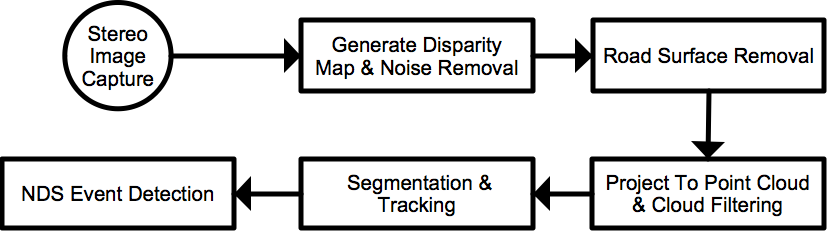
\includegraphics[width=0.42\textwidth]{text/figures/systemForeslag4.png}
  \captionof{figure}{Overview of the methods used in the proposed NDS system.}
  \label{systemOverview::systemOverview}
\end{figure}

%The road surface is removed using the detected line in a corresponding v-disparity. The remaining pixels are considered vehicle candidate pixels. These pixels are projected into 3D world coordinates and outliers are removed. Segmentation into clusters is done by grouping points that are close neighbors into the same clusters. Each sufficiently big cluster is regarded as a detected vehicle. Finally, the detected vehicles are tracked and NDS event are detected and logged in a drive analysis report. \\[5pt]

\textbf{Generate Disparity Map \& Noise Removal}\\
A disparity map is generated using OpenCV's SGBM implementation. For noise reduction, a LR-RL consistency check is done \cite{HirschmullerRLandSGBM}. In case of a disparity differences in the consistency check, the lowest value is selected as the output pixel. A temporal consistency check assumes that a pixel's disparity value does not change erratically between frames. Finally, a monocular color check removes pixels from extremely light and dark regions.

\textbf{Road Surface Removal}\\
The road surface is found by searching for the most significant line in the V-disparity using RANSAC. Additionally, the line parameters are filtered using a Kalman filter to smooth out faulty road surface detections. The parameters are then used to remove pixels for everything not above the road surface. The remaining pixels are considered vehicle candidate disparity pixels. In Figure \ref{fig:methods::disparity:dispEx1:postVdisp} the left input image and the vehicle candidate disparity map are shown.

\begin{figure}[H]
  \centering
  \begin{tabular}{cc}
    \subfloat[A rectified image captured]{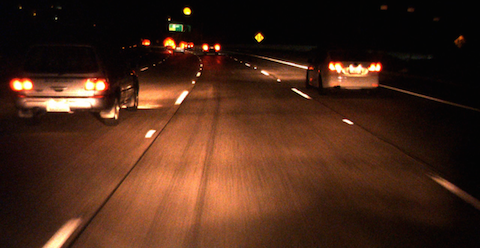
\includegraphics[width=0.22\textwidth]{text/figures/methods/dispEx1/inputL.png} \label{fig:methods::disparity:dispEx1:inputl}} &
    \subfloat[Noise reduced disparity image.]{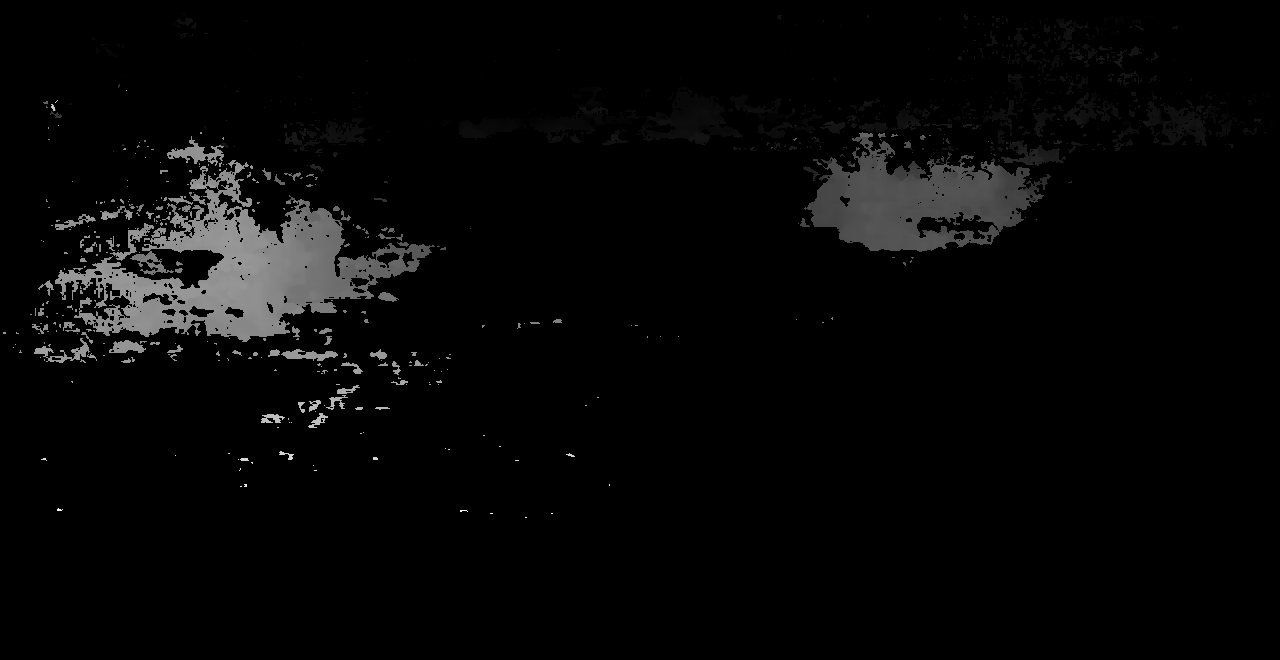
\includegraphics[width=0.22\textwidth]{text/figures/methods/dispEx1/postVDisp.png} \label{fig:methods::disparity:dispEx1:postVDisp}}\\
  \end{tabular}
  \caption{Results after Generate Disparity Map \& Noise Removal and Road Surface Removal.}
\label{fig:methods::disparity:dispEx1:postVdisp}
\end{figure}

\textbf{Project To Point Cloud \& Cloud Filtering}\\
Using the camera's focal length $f$(in pixels) and it's baseline $b$(in meters), along with the calculated disparity $d$(in pixels), the actual distance $z$ to objects in the camera's view can be found. The remaining $x$ and $y$ component of the world coordinate are found using the column and row index of the disparity pixel.% \\[5pt]

\textbf{Segmentation \& Tracking}\\
The acquired point clouds are post processed using a band-bass filter to remove near and distant points, downsampled using a voxel grid, and removing outliers. Clusters are found by creating k-d tree, and for each point finding neighbors within a specified radius. The clusters center point is used for nearest neighbor tracking between frame and used to determine the distance from ego vehicle to detected vehicle.


\textbf{NDS Event Detection}\\
For compensating for the subject vehicle's ego-motion while e.g. approaching an intersection, we utilize the \textit{LIBVISO2: C++ Library for Visual Odometry 2} \cite{Geiger2011IV}. NDS events are detected by looking at the movement history of other vehicles with regard to the ego vehicle. 

\begin{figure}[H]
  \centering
  \begin{tabular}{cc}
    \subfloat[]{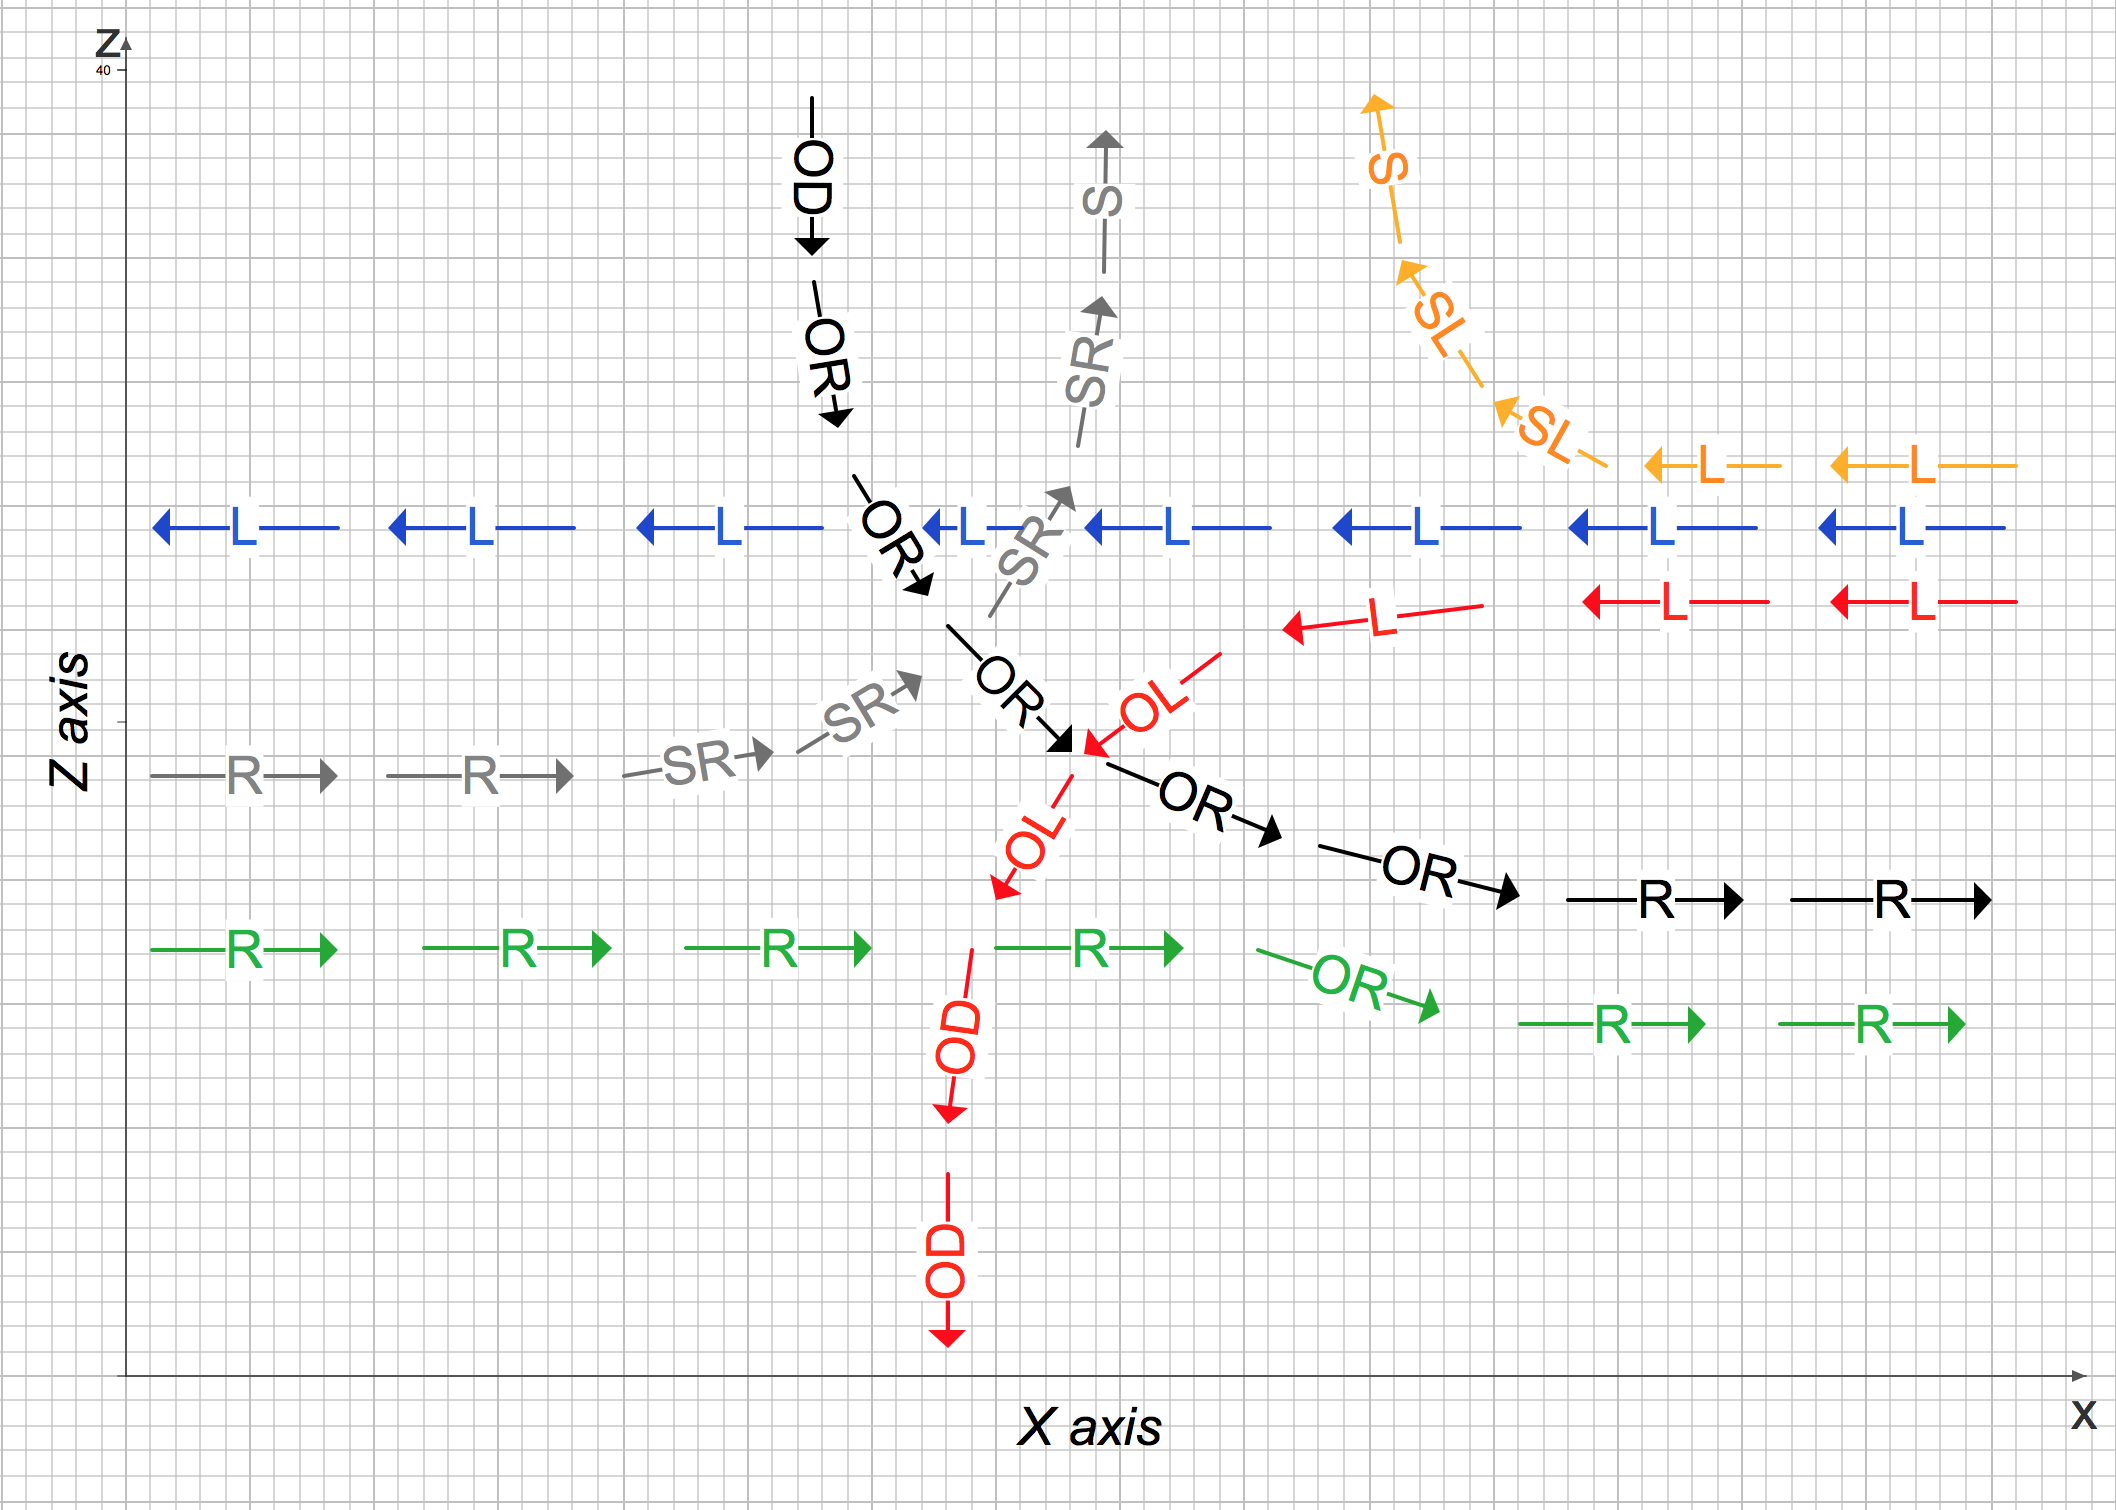
\includegraphics[width=0.22\textwidth]{text/figures/methods/intersectionVoting.png} \label{fig:methods::intersectionVoting}} &
    \subfloat[]{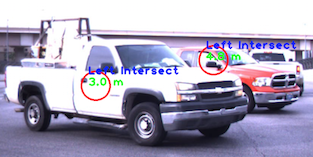
\includegraphics[width=0.22\textwidth]{text/figures/methods/frame2.png} \label{fig:methods::disparity:dispEx1:postVDisp}}\\
  \end{tabular}
  \caption{(a) Illustration of various movements that are detected by the system. (b) NDS detection example.}
\label{fig:methods::disparity:dispEx1:postVdisp}
\end{figure}

For all detected vehicles, individual frame to frame movements are categorized to form a a histogram of events for determining which NDS events have occurred. An example of such a histogram is seen in Figure \ref{methods::histogram}.
\begin{figure}[H]
\centering
     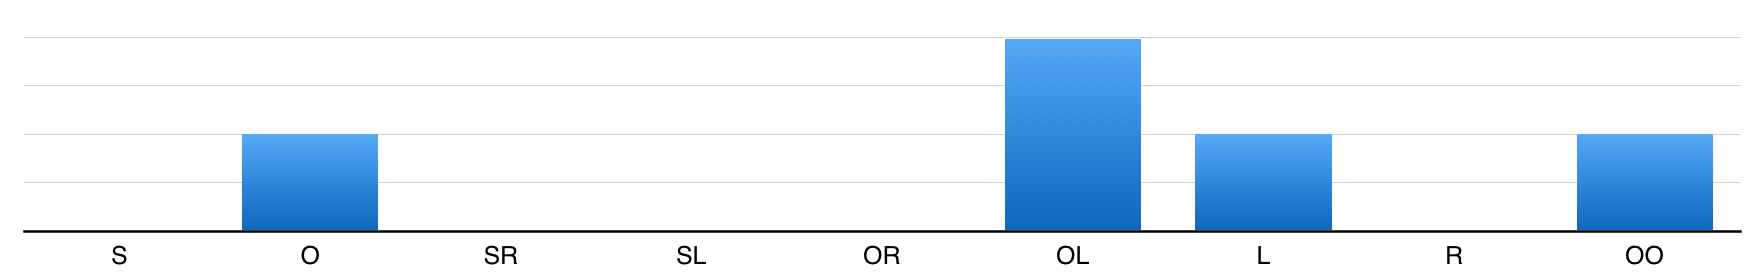
\includegraphics[width=0.4\textwidth]{text/figures/methods/eventHistogram.png}
     \caption{Example of histogram of detected movements.}
     \label{methods::histogram}
\end{figure}
\end{multicols}

